\section{Pistepilvien visualisointi}\label{kirjallisuus}

Tässä luvussa selvitetään, mitä haasteita pistepilvien ominaisuudet asettavat visualisoinnissa käytetyille tietorakenteille ja algoritmeille. Lisäksi tutustutaan alan julkaisuihin, joilla haasteisiin pyritään vastaamaan.

\subsection{Pistepilvien visualisoinnin haasteet}

Suurin haaste pistepilvien käsittelyssä ja visualisoinnissa on niiden koko. Nykyaikainen laserkeilain, kuten luvussa \ref{laserkeilaimet} esitetty Leica Geosystemsin RTC360, tuottaa pistepilven, jossa on satoja miljoonia pisteitä. Kun tällaisella keilaimella tehdään useita keilauksia, on pisteiden määrä valtava. Oletetaan esimerkiksi, että suuressa projektissa käytetään pistepilviä, joissa on yhteensä miljardi pistettä. Kun koordinaatit tallennetaan kolmella nelitavuisella liukuluvuulla ja värit RGB-muodossa kolmella tavulla ja lisätään perään vielä yksi täytetavu, voidaan yksi pilven piste esittää 16:lla tavulla. Miljardin pisteen pilvi olisi siis kooltaan 16 gigatavua mahdollisen metadatan lisäksi. Tämän kokoista pilveä ei haluta pitää kerralla keskusmuistissa, vaan pisteitä haetaan levyltä muistiin vain tarvittaessa. 

Pisteiden tallentaminen levylle aiheuttaa kuitenkin ongelmia tiedonsiirron hitauden takia, sillä tiedonsiirtonopeus kiintolevyltä on jopa kaksi kertaluokkaa hitaampi kuin keskusmuistista. Ongelman ratkaisemiseksi käytetään usein ulkoisen muistin algoritmeja \engl{out-of-core algorithm}, jotka lataavat pisteitä levyltä muistiin isoissa palasissa, mikä on huomattavasti nopeampaa kuin yksittäisten pisteiden lataaminen. \cite{scheiblauer} 

Pistepilvien koon vuoksi ei ole realistista olettaa, että kaikki pisteet voitaisiin renderöidä reaaliajassa.\footnote{Miellyttävän käyttökokemuksen takaamiseksi pitäisi ruutu päivittää vähintään kymmenen kertaa sekunnissa.} Tästä syystä on kehitetty erilaisia tekniikoita pistepilven harventamiseen ja osittaiseen renderöintiin. Yksinkertainen tapa harventaa pistepilveä on jakaa sen peittämä alue niin kutsuttuihin vokseleihin \engl{volume element, voxel}, eli säännöllisiin kuutioihin, ja visualisoimalla vain yksi piste kustakin vokselista. Pilven harventaminen kuitenkin aiheuttaa yksityiskohtien katoamista pilvestä, joten sitä täytyy käyttää sovelluskohteesta riippuen maltillisesti. 

Toinen keino vähentää visualisoitavien pisteiden määrää on määrittää pistepilvelle tarkkuustasot \engl{level-of-detail, LOD}. Tarkkuustasot mahdollistavat pistepilven astettaisen tarkentamisen karkeasta yleiskuvasta yksityiskohtiin. Usein interaktiivisissa ohjelmistoissa korkean ruudunpäivitystaajuuden ylläpitäminen vaatii sitä, että pistepilvi renderöidään matalimmalla tarkkuudella esimerkiksi käyttäjän pyörittäessä näkymää. Toisaalta kun kamera pysähtyy paikalleen, voidaan renderöintiin käyttää enemmän aikaa ja pistepilveä tarkentaa.

\subsection{Hierarkiset tietorakenteet}\label{tietorakenteet}

Edellä mainittuihin haasteisiin on otettu kantaa laajalti alan julkaisuissa. Lupaavin tekniikka tarkkuustasojen muodostamiseen, ulkoisen muistin käyttöön ja pistepilvien harventamiseen näyttää olevan pistepilven jakaminen hierarkiseen tietorakenteeseen. Ajatuksena on, ettei kaikkia pisteitä tarvitse käydä läpi jokaisella ruudunpäivityksellä, vaan hierarkian yläpäässä on karkein tarkkuustaso ja alaspäin kulkiessa tarkkuus kasvaa.  

Esitellään seuraavaksi muutama kiinnostava hierarkinen tietorakenne. Aihealueen pioneerityönä pidetään Rusinkiewiczin ja Levoyn Qsplatia, joka onkin antanut vaikutteita uudemmille tietorakenteille. Dachsbacher et al. esittelivät peräkkäispistepuut, jotka voidaan renderöidä hyvin nopeasti näytönohjaimella. Viime vuosina pistepilvien visualisoinnin tutkimuksen kirkkainta kärkeä on edustanut Wienin teknillisen yliopiston tietokonegrafiikan tutkimusyksikkö. Tämän tutkielman päälähteinä käytetään Claus Scheiblauerin ja Markus Schützin julkaisuja sisäkkäispistepuista.

\subsubsection{Qsplat}
Yksi ensimmäisistä pistedatan visualisointiin käytetyistä hierarkisista tietorakenteista on Rusinkiewiczin ja Levoyn esittämä QSplat, joka on kehitetty polygoniverkon visualisointiin pisteiden avulla. Tietorakenne muodostetaan kolmioidusta mallista, jossa kolmioiden normaalit tunnetaan, joten se ei suoraan sovellu raa'an pistepilvidatan käsittelyyn.\footnote{Itse asiassa Rusinkiewicz ja Levoy käyttivät laserkeilatusta pistepilvestä muodostettua kolmioverkkoa, jonka tietorakenne esitti yksinkertaistettuna pistedatana.} QSplatissa on käytetty kuitenkin monia kiinnostavia tekniikoita, joita voi hyödyntää pistepilvien käsittelyssä. \cite{qsplat}

QSplat perustuu puurakenteeseen, jonka solmuissa on rajauspalloja \engl{bounding sphere}. Pallot jakavat avaruutta rekursiivisesti pienempiin osiin siten, että juuren pallo sisältää kaikki kolmiot ja jokainen sisäinen solmu jakaa avaruuden keskimäärin neljään osaan. Puun latva saavutetaan, kun avaruuden jakamisen seurauksena jäljelle jää yksi kolmio. Siitä muodostetaan lehtisolmu, jonka rajauspallo sisältää koko kolmion. Puun visualisointi onnistuu piirtämällä jokaisen pallon kohdalle sopivan kokoinen täplä \engl{splat}. Puurakenne mahdollistaa myös tehokkaan pisteiden karsimisen. Jos solmun pallo ei ole näkökentässä, eivät sen lapsetkaan ole ja haaraa ei tarvitse käydä läpi. \cite{qsplat}

Puurakenne tallennetaan levylle leveysjärjestyksessä \engl{breadth-first}. Tämän ansiosta puun tasot muodostavat luonnolliset tarkkuustasot: juurisolmun pallo esittää koko mallia, ensimmäinen taso sisältää muutaman pienemmän pallon, ja niin edelleen. Kun tällainen tiedoston sisäinen rakenne yhdistetään ulkoisen muistin tekniikoihin, voidaan täplien piirtäminen aloittaa heti, kun tarpeeksi puun solmuja on ladattu levyltä muistiin.\footnote{Rusinkiewicz ja Levoy päättävät ruudulle projisoitujen täplien koon perusteella kuinka syvälle puussa tulee edetä.} Puun rakennetta on havainnollistettu kuvassa \ref{tarkkuustasot}. \cite{qsplat}

\begin{figure}
    \centering
    \subfile{fig/puuntasot.tex}
    \caption{Puun läpikäyntijärjestys (punainen katkoviiva) muodostaa luonnolliset tarkkuustasot}
    \label{tarkkuustasot}
\end{figure}

Toinen hyödyllinen QSplatissa käytetty tekniikka on koordinaattien kvantisointi \engl{quantization}. Kun tarkkuudesta voidaan tinkiä, solmujen pallojen absoluuttisia koordinaatteja ei tallenneta, vaan niiden sijainti ilmaistaan suhteessa vanhempiinsa. Pallon säteen ja keskipisteen suhteellisen poikkeaman ilmaisemiseen käytetään vain 13:a arvoa. Pallon säde $r$ voi olla välillä $[\frac{1}{13}, \frac{13}{13}]$ ja samaten keskipisteen suhteellisen poikkeaman $x, y$ ja $z$ -koordinaatit ovat vanhemman pallon läpimitan kolmastoistaosan monikertoja. Kun vielä hylätään vanhemman pallon ulkopuolella olevat keskipisteet ja käytetään hakutaulua, voidaan pallon sijainti esittää vain 13:lla bitillä, kun normaali liukulukuesitys vaatisi vähintään 16 tavua. \cite{qsplat}

QSplat onnistui renderöimään 1,5-2,5 miljoonaa pistettä sekunnissa, mikä on sen aikaisella laitteistolla erinomainen tulos \cite{qsplat}. Kuten sanottu, se ei sellaisenaan kuitenkaan sovellu laserkeilattujen pistepilvien käsittelyyn. Pistepilvien pisteiden normaaleja ei yleensä tiedetä, joten ne pitäisi esiprosessointivaiheessa selvittää esimerkiksi luvussa \ref{workflow} esitetyllä tekniikalla. 

Toisena ongelmana voidaan pitää tapaa, jolla mallin kolmioita esitetään palloina. Tietorakenteeseen luodaan nimittäin uutta dataa, kun lehtisolmuihin tallennettujen, yhden kolmion sisältävien pallojen lisäksi ylemmillä tasoilla on keinotekoisia, monia kolmioita kuvaavia palloja. QSplat tarjoaa kuitenkin monia tekniikoita, joita pistepilviä käsittelevässä tietorakenteessa voidaan hyödyntää, kuten hierarkinen rakenne ja koordinaattien suhteellinen esitystapa.

\subsubsection{Peräkkäispistepuut}
Dachsbacher et al. esittelevät niin kutstutun peräkkäispistepuun \engl{sequential point tree}, jossa pisteet on aluksi järjestetty samaan tapaan pallopuuhun kuin QSplatissa. Pisteet sijaitsevat puun lehtisolmuissa ja sisäsolmuissa säilytetään täpliä, jotka juuri ja juuri peittävät solmun lasten rajauspallot. Täplien väri määräytyy lapsisolmujen värien keskiarvolla. \cite{spt}

Jokaiseen puun solmuun on virhelaskelmien perusteella lisätty rajat katseluetäisyydelle, jolla solmu valitaan visualisoitavaksi. Visualisointivaiheessa hierarkia litistetään taulukoksi, joka voidaan syöttää suoraan näytönohjaimelle. Näytönohjain käy taulukkoa läpi ja valikoi sopivat solmut, joiden perusteella täpliä piirretään ruudulle. \cite{spt}

Peräkkäispistepuut voidaan renderöidä nopeasti näytönohjaimen käytön ansiosta, mutta niissä on myös heikkouksia. Tietorakenteen vaatimuksena on, että kaikki data mahtuu näytönohjaimen muistiin. Näin on vain pienillä malleilla ja tilannetta pahentaa se, että peräkkäispistepuut eivät ole kovin säästäväisiä muistin suhteen. Hierarkian jokaisessa sisäsolmussa luodaan lisää dataa, kun lapsisolmujen unionia kuvataan täplän sijainnilla ja koolla, sekä keskimääräisellä värillä.

Wimmer ja Scheiblauer esittävät parannuksia peräkkäispistepuihin. Uusien täplien luomisen sijaan puun sisäsolmuissa valitaan lapsisolmuista edustaja, joka parhaiten kuvaa sisäsolmun esittämää avaruuden osaa. Tämä on tärkeä huomio, sillä käsiteltäessä massiivisia pistepilviä tulisi välttää ylimääräisen datan luomista. Hierarkiasta muodostetaan tarkkuustasot siten, että alemmat tarkkuustasot sisältyvät ylempiin tasoihin ja visualisoitaessa oikea tarkkuustaso valitaan täplien koon ja katseluetäisyyden perusteella. Solmua vastaavan täplän koko määräytyy siitä, kuinka syvällä hierarkiassa se on. Wimmer ja Scheiblauer kutsuvat tätä rakennetta muistioptimoiduksi peräkkäispistepuuksi. \engl{memory optimized sequential point tree, MOSPT} \cite{ip} %Kun hierarkian läpikäymistä jatketaan niin pitkälle, että solmujen täplät ovat yhden pikselin kokoisia, ei lopputulokseen jää aukkoja. \cite{ip}

\subsubsection{Sisäkkäispistepuut}
\begin{figure}
    \centering
    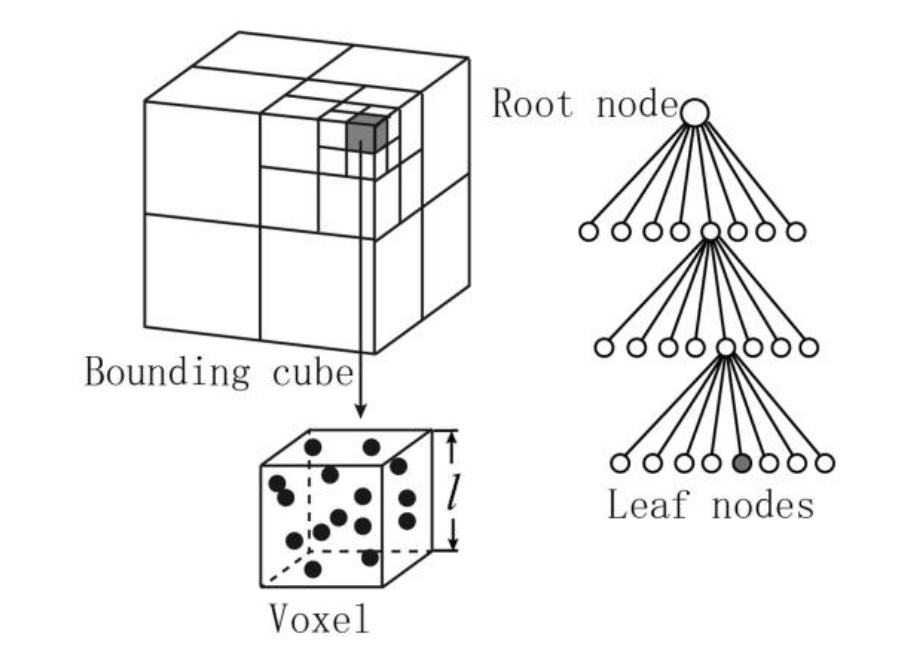
\includegraphics[width=0.5\paperwidth]{img/octree.png}
    \label{octree}
    \caption{Oktettipuun juurisolmu sisältää kaikki pisteet sisältävän rajauslaatikon. Jokainen sisäsolmu jakaa rajauslaatikkonsa kahdeksaan osaan. Kuva: \cite{octreekuva}}
\end{figure}

Wimmer ja Scheiblauer kritisoivat muistioptimoituja peräkkäispistepuita siitä, että ne eivät tue näkökentän ulkopuolisten pisteiden tehokasta karsimista ja siitä, ettei muistioptimointi yksinään riittänyt poistamaan tarvetta ulkoisen muistin algoritmeille. Ratkaisuksi he esittivät sisäkkäisiä oktettipuita \engl{nested octree}. Oktettipuu\footnote{Tätä suomennosta käyttää esimerkiksi Davidsson \cite{oktettipuu}. Vaihtoehtoinen suomennos on kahdeksanpuu.} on yksinkertainen avaruutta rekursiivisesti jakava tietorakenne, jonka jokainen sisäsolmu jakaa kuvaamansa avaruuden kahdeksaan samankokoiseen osaan. Oktettipuun rakennetta on havainnollistettu kuvassa \ref{octreekuva}. 

Wimmerin ja Scheiblauerin tietorakenteessa oktettipuita on kahdessa tasossa. Ulompaa oktettipuuta käytetään avaruuden jakamiseen, sen tehokkaseen läpikäymiseen ja näkökentän ulkopuolisten alueiden karsimiseen. Ulomman puun jokainen solmu sisältää yhden sisemmän oktettipuun, joka vastaa samaa avaruuden osaa, kuin ulkoisen puun solmu. Pisteet sijoitetaan sisempiin puihin, yksi jokaiseen solmuun. \cite{ip}

\begin{figure}
    \centering
    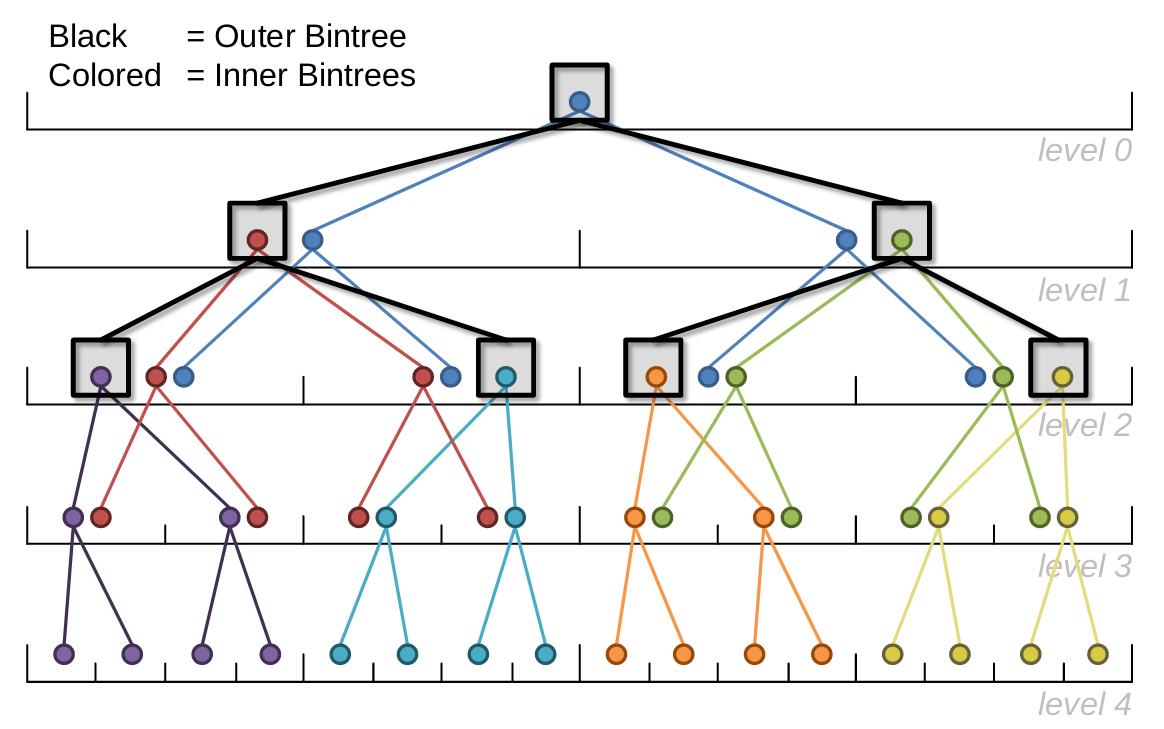
\includegraphics[width=0.6\paperwidth]{img/nested.png}
    \caption{Sisäkkäinen binääripuu, jossa sekä ulomman, että sisempien puiden syvyys on kolme. Ulompaa puuta kuvaavat mustat neliöt ja sisempää värikkäät ympyrät. Puista muodostuu viisi tarkkuustasoa. Kuva: \cite{scheiblauer}}
    \label{nested}
\end{figure}

Sisäkkäisistä oktettipuista luodaan tarkkuustasot siten, että sisemmistä puista kerätään pisteitä ulomman puun tasojen mukaan. Tarkkuustasoon kuuluvat pisteet sijaitsevat siis ulomman puun samalla tasolla, mutta useiden sisempien puiden eri tasoilla. Tarkkuustasojen muodostumista on havainnollistettu kuvassa \ref{nested}. Puut tallennetaan levylle tarkkuustaso kerrallaan, mikä mahdollistaa ulkoisen muistin algoritmien käytön. Visualisoitaessa tarvitsee levyltä lukea pisteitä vain haluttuun tarkkuustasoon asti, eikä loppuja pisteitä tarvitse ladata muistiin. \cite{ip}

Scheiblauer jalostaa sisäkkäisten oktettipuiden ideaa väitöskirjassaan esittelemällä muokattavat sisäkkäiset oktettipuut \engl{modifiable nested octree, MNO}. Jos edellä esiteltyjä sisäkkäisiä oktettipuita halutaan muokata rakentamisen jälkeen, on sisemmät puut rakennettava ja muokattu hierarkia tallennettava levylle uudestaan. Nimensä mukaisesti MNO mahdollistaa tehokkaan pisteiden lisäämisen ja poistamisen. \cite{scheiblauer}  

MNO:n rakenne eroaa sisäkkäisistä oktettipuista siten, että sisemmät puut korvataan säännöllisillä kolmiulotteisilla ruudukoilla, joihin pisteet tallennetaan. MNO:n rakentaminen alkaa juurisolmusta, joka vastaa kaikki pisteet peittävää avaruutta. Solmun sisältämä ruudukko jakaa solmua kuvaavan avaruuden osan $128^3 = 2 097 152$ soluun. Pisteitä lisätään puuhun yksi kerrallaan niin, että jokaiseen ruudukon soluun mahtuu vain yksi piste. Jos solu on varattu, sijoitetaan piste ylimääräiseen taulukkoon odottamaan, että vastaavia pisteitä kertyy tarpeeksi, jotta olisi järkevää luoda uusia solmuja puuhun. Kun ennaltamäärätty vähimmäismäärä pisteitä on kertynyt ylimääräisten pisteiden taulukkoon, luodaan ruudukon sisältävälle solulle lapsisolmuja ja sijoitetaan ylimääräiset pisteet niihin. Ruudukkoon sijoitettavien pisteiden määrälle on hyvä asettaa myös yläraja. \cite{scheiblauer}

Jokainen tietorakenteen solmu tallennetaan omaan tiedostoonsa levylle, josta niitä ladataan muistiin visualisointivaiheessa tarvittaessa. Renderöintialgoritmiin kuuluu käyttäjän asettama pistebudjetti, joka asettaa ylärajan yhdessä ruudunpäivityksessä piirrettävien pisteiden määrälle.\footnote{Scheiblauer testasi pistepilvivisualisoijaansa asettamalla rajan vain sataantuhanteen pisteeseen.} Tätä rajaa säätämällä käyttäjä saa jonkinlaisen kontrollin ruudunpäivitystaajuuden suhteen. \cite{scheiblauer}

Tiedostorakenne mahdollistaa hierarkian tehokkaan muokkaamisen. Lisättäessä uusia pisteitä MNO:hon tarkastetaan ensin, sijoittuuko se juurisolmun kuvaamaan avaruuden osaan. Jos näin on, onnistuu lisääminen kuten rakennusvaiheessa. Muussa tapauksessa juurisolmulle luodaan vanhempia kunnes jokin niistä muodostaa tarvittavan kokoisen avaruuden, ja piste lisätään sen ruudukkoon. Kun puun vanhan juuren yläpuolelle luodaan uusia solmuja, jää niiden ruudukot vajaaksi. Tällöin alemmista solmuista nostetaan pisteitä ylöspäin niin kauan, kunnes vajaita ruudukoita on vain lehtisolmuissa. Pisteiden poistaminen puusta on triviaalia, kun sisäsolmuihin mahdollisesti jäävät tyhjät ruudukot täytetään kuten pisteitä lisättäessä. \cite{scheiblauer}

Scheiblauer oli ottanut MNO:ta kehittäessään vaikutteita Michael Wandin et al. esittämästä oktettipuusta, jonka sisäsolmuihin kuuluu myös ruudukko. Pisteet tallennetaan kuitenkin ruudukon sijaan lehtisolmuihin joihin mahtuu kuhunkin enintään satatuhatta pistettä. Sisäsolmuissa pidetään kopiota yhdestä niiden läpi kulkeneesta pisteestä ja tarkkustasot muodostetaan näistä sisäsolmujen pisteistä. Wandin et al. tietorakenne käyttää MNO:n tapaan ulkoista muistia ja mahdollistaa tehokkaat lisäys- ja poisto-operaatiot. \cite{wand}

Markus Schütz jatkoi Wimmerin ja Scheiblauerin työtä esittelemällä opinnäytetyössään verkkoselaimessa ajettavan Potree-nimisen pistepilvivisualisoijan. Potreen käyttämä tietorakenne perustuu Scheiblauerin muokattaviin sisäkkäisiin oktettipuihin, mutta hierarkian rakennusvaiheessa kiinnitetään huomiota pisteiden tasaiseen jakautumiseen solmujen välille. Oktettipuun sisäsolmujen ruudukoihin hyväksytään uusia pisteitä vain, jos ne ovat tarpeeksi kaukana muista ruudukon pisteistä. Lehtisolmut hyväksyvät ennaltamäärättyyn rajaan saakka kaikki pisteet, kunnes ne muutetaan sisäsolmuiksi ja liian lähekkäin olevat pisteet jaetaan uusien lapsisolmujen kesken. \cite{potree}

Potree käyttää ulkoista muistia tehokkaasti ja pystyy käsittelemään jopa 640 miljardia pistettä sisältäviä pistepilviä.\footnote{Kyseinen pistepilvi (Actueel Hoogtebestand Nederland, ANH2, \url{http://ahn2.pointclouds.nl/}) kuvaa koko Alankomaiden valtiota ja se vaatii 7,68 teratavua tallennustilaa. Potreen tietorakenteessa pistepilvi jakautui 13:lle tasolle ja 38:aan miljoonaan solmuun.} Rakennusvaiheessa oktettipuun solmuja tallennetaan tasaisin väliajoin levylle, jottei muisti täyttyisi. Kun jokainen solmu tallennetaan omaan tiedostoonsa, on yksittäisten solmujen tallentaminen ja lukeminen levyltä helppoa. Massiivisia pistepilviä kuvaavat hierarkiatkin voivat olla satojen megatavujen kokoisia. Schütz ratkaisee suurten hierarkioiden nopean lataamisen verkon yli jakamalla senkin puurakenteeseen. Näin voidaan välttää sekä turhien pisteiden, että näkökentän ulkopuolella olevien hierarkian haarojen lataaminen muistiin. \cite{potree}

Potreen visualisointialgoritmi priorisoi niitä hierarkian solmuja, jotka ovat lähellä katselupistettä ja joiden kuvaruudulle projisoitu koko on suurin. Renderöinnin suorituskykyä voidaan säädellä Scheiblauerin toteutuksen mukaisesti käyttäjän asettamalla pistebudjetilla. Schütz on kehittänyt Potreehen myös näytönohjaimella ajettavan algoritmin mukautuvaan pisteiden koon määrittämiseen; pistepilven harvemmissa osissa piirretään pisteet suurempina, jottei reikiä esiintyisi. \cite{potree}

\subsubsection{kd-puut}
Suosittujen oktettipuiden lisäksi on pistepilvien visualisoinnissa käytetty kd-puita \engl{k-dimensional tree, kd-tree}\footnote{Kolmiulotteisten mallien visualisointiin käytetyissä kd-puissa luonnollisesti $k=3$}. Oktettipuusta poiketen kd-puut eivät jaa pistepilveä yhtäsuuren tilavuuden omaaviin osiin, vaan jokainen solmu jakaa kuvaamansa alueen kahtia niin, että tilanjakotason molemmille puolille jää yhtä monta pistettä. Tätä varten pisteet on järjestettävä, mikä pidentää puun rakennusaikaa. Toisaalta tietorakenteen siirtely kiintolevyltä muistiin ja sieltä näytönohjaimelle on helpompaa, kun puu on tasapainoinen, eli kaikki solmut ovat saman kokoisia. \cite{richter}

Richter et al. kehittivät massiivisten ulkoilmakeilausten visualisointiin kd-puuhun perustuvan pistepilvirenderöijän, joka käytti luokiteltua pistepilvidataa. Pisteet oli jaettu objektiluokkiin, kuten kasvillisuus, vesi tai rakennus, joille jokaiselle rakennettiin oma kd-puu. Renderöintivaiheessa kd-puista lähetetään solmuja näytönohjaimelle niiden kuvaruudulle projisoidun koon määräämässä järjestyksessä niin, että jokaisella objektiluokalla oli oma rajansa muistinkäytölle. \cite{richter}

Futterlieb et al. käyttivät samankaltaista kd-puuta luokittelemattomalle pistedatalle. Edellä mainitusta toteutuksesta poiketen tarkkuustaso valitaan etsimällä puusta yksi taso, jolta saadaan renderöityä sopiva määrä pisteitä. Varmistaakseen, että ruudulle saadaan aina jonkinlainen tarkkuustaso renderöityä nopeasti Futterlieb et al. pitivät kahta miljoonaa pistettä näytönohjaimen muistissa jatkuvasti riippumatta siitä, olivatko ne näkyvissä. \cite{smooth}

\subsection{Ei-hierarkiset tekniikat}

%\subsubsection{Jatkuvat tarkkustasot}
Pistepilvistä voi muodostaa tarkkuustasoja myös ilman hierarkista tietorakennetta. Markus Schütz et al. esittivät virtuaalitodellisuuslaseille suunnatun pistepilvirenderöijän, joka hierarkian muodostamisen sijaan käy koko pistepilveä läpi ja muodostaa siitä noin viiden ruudun välein uuden, sopivan tiheästi näytteistetyn osajoukon. Tämä jatkuviksi tarkkuustasoiksi \engl{continuous LOD} kutsuttu tekniikka ei siis jaa pisteitä tietorakenteen solmuihin, joilla on diskreetit tarkkuustasot, vaan pisteiden etäisyys toisistaan vaihtelee sen perusteella, kuinka kaukana ne ovat kamerasta. \cite{clod}

\begin{figure}
    \centering
    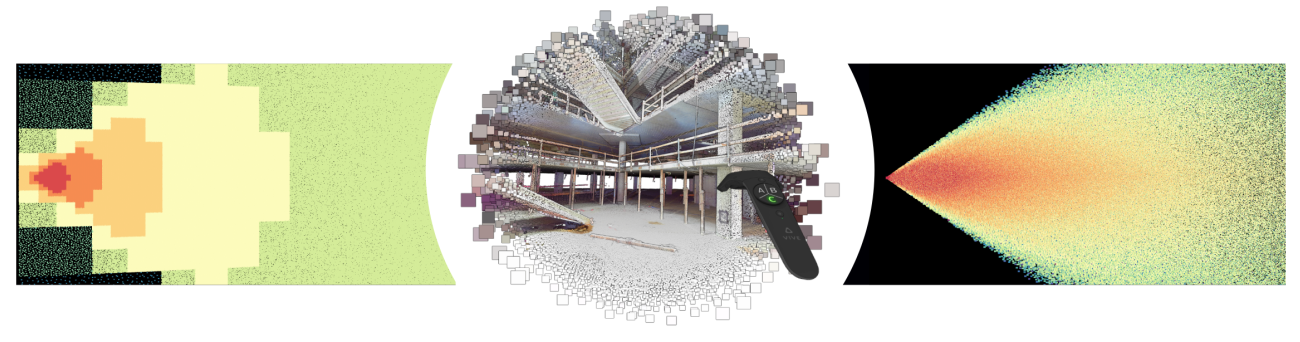
\includegraphics[width=\textwidth]{img/clod.png}
    \caption{Vasemmalla pistepilvi on jaettu diskreetteihin tarkkuustasoihin, joiden välillä on selkeät rajat. Oikealla on käytetty jatkuvia tarkkuustasoja ja pisteet sulautuvat siististi kuvaan. Kuva: \cite{clod}}
    \label{img:clod}
\end{figure}

Jatkuvat tarkkuustasot ratkaisevat hierarkisia tietorakenteita käytettäessä usein esiintyvän ongelman diskreettien tarkkuustasojen näkyvistä rajoista. Renderöidyssä kuvassa ei näy selkeitä eroja matalalla ja korkeammalla tarkkuudella renderöityjen solmujen välillä kun tarkkuus laskee vähitellen kamerasta poispäin. Kuvassa \ref{img:clod} vasemmalla on havainnollistettu diskreettejä tarkkuustasoja ja oikealla jatkuvia tarkkuustasoja.